\documentclass[10pt]{article}

\addtolength{\textwidth}{1.3in}
\addtolength{\oddsidemargin}{-.65in} %left margin
\addtolength{\evensidemargin}{-.65in}
\setlength{\textheight}{9in}
\setlength{\topmargin}{-.5in}
\setlength{\headheight}{0.0in}
\setlength{\footskip}{.375in}
\renewcommand{\baselinestretch}{1.0}
%\linespread{1.5}
\usepackage{setspace}
\doublespacing

\usepackage{titling}

\usepackage[pdftex]{graphicx}

\usepackage[usenames,dvipsnames]{color}
\usepackage{cite}
\usepackage{times, verbatim,bm,pifont,pdfsync}
\usepackage{caption}
\usepackage{subcaption}

\usepackage{tikz}
\tikzset{
% Two node styles for game trees: solid and hollow
solid node/.style={circle,draw,inner sep=1.5,fill=black},
hollow node/.style={circle,draw,inner sep=1.5,fill=white}
%non node/.style={circle,draw,inner sep=.1,fill=black}
}

% disables chapter, section and subsection numbering
%\setcounter{secnumdepth}{-1} 

\usepackage{amsbsy,amssymb, amsmath, amsthm, MnSymbol,bbding}
\usepackage[hang,flushmargin]{footmisc} 

\usepackage[pdftex,
bookmarks=true,
bookmarksnumbered=false,
pdfview=fitH,
bookmarksopen=true]{hyperref}

\newtheorem{definition}{Definition}
\newtheorem{theorem}{Theorem}
\newtheorem{lemma}{Lemma}
\newtheorem*{lemma*}{Lemma}
\newtheorem{corollary}{Corollary}
\newtheorem{assumption}{Assumption}
\newtheorem{fact}{Fact}
\newtheorem{result}{Result}

\newcommand{\ve}{\theta}
\newcommand{\ta}{\theta}
\newcommand{\ov}{\overline}
\newcommand{\un}{\underline}
\newcommand{\al}{\alpha}
\newcommand{\Ta}{\Theta}
\newcommand{\expect}{\mathbb{E}}
\newcommand{\Bt}{B(\bm{\tau^a})}
\newcommand{\bta}{\bm{\tau^a}}
\newcommand{\btad}{\bm{\tau^{ad}}}
\newcommand{\bte}{\bm{\tau^E}}
\newcommand{\btn}{\bm{\tau^n}}
\newcommand{\ga}{\gamma}


\begin{document}
\title{\vskip-0.6in Temporary Trade Barriers: When Will They End?}%\protect\footnote{Formerly circulated under the title }}
\thanksmarkseries{alph}
\author{Kristy Buzard\thanks{Syracuse University, Economics Department, 110 Eggers Hall, Syracuse, NY 13244, USA. Ph: 315-443-4079. Fax: 315-443-3717. Email: kbuzard@syr.edu. http://faculty.maxwell.syr.edu/kbuzard.}} 
\date{\vskip-.1in \today}
\maketitle

\begin{center} {\bf Abstract} \end{center}

\begin{quote}
{Abstract

\textit{JEL classification:} D72, F13, F55 \\
\textit{Keywords:} temporary trade barriers, WTO, disputes, lobbying, political economy}
\end{quote}

\bigskip
\section{Introduction}



\subsection{Related Literature}
\textbf{WILL NEED MAJOR OVERHAUL}

This work rests on the foundation of Grossman and Helpman's (1994) `Protection for Sale.' Two related papers `Trade Wars and Trade Talks' (Grossman and Helpman (1995b)) and `The Politics of Free-Trade Agreements' (Grossman and Helpman (1995a)) first employed the PFS approach in the study of trade agreements. The first considers ``Trade Wars'' and ``Trade Talks'' separately, whereas my approach views the ``Trade War'' as a crucial subgame. The model of preferential trade agreements (Grossman and Helpman (1995a)), although treating the government as a unitary actor, is closer to this approach.

Another related literature considers the impact of exogenously-determined political uncertainty on the potential for trade cooperation. These studies (e.g. Feenstra and Lewis (1991); Milner and Rosendorff (2001); Bagwell and Staiger (2005); Beshkar (2010); Horn, Maggi and Staiger (2010); Beshkar and Bond (2012)) derive various implications for the design of international trade agreements using a Baldwin (1987)-style government welfare function with exogenous shocks to the political-pressure parameter. 

Since trade policies are overwhelmingly determined in the context of trade agreements, it is useful to have a framework to bring together the endogenous political pressure of PFS-style modeling with the trade agreements approach. The government objective function introduced in this paper is intended to be a bridge between the two. This objective function starts from the Baldwin (1987) government objective function and adds flexibility: the weight the legislature places on profits is endogenous (PFS), potentially non-linear (Findlay and Wellisz 1982; Dixit, Grossman and Helpman 1997) and stochastic. Buzard (2016) is an example of how this modeling approach can be used to integrate  endogenous political activity and exogenous shocks into the analysis of questions regarding optimal trade agreement design.

Modeling the objective function so closely on the standard in the trade agreements literature allows for direct comparisons to the large body of work that studies exogenous shocks only, revealing cleanly the effects of the addition of endogenous lobbying. To preview, this model is closest to that of Bagwell and Staiger (2005), with two main changes: in place of their unitary government signing a trade agreement and having different preferences ex-ante and ex-post, this model has two branches of government with differing preferences, where the political economy weights of the legislature are determined endogenously.
		
Mansfield, Milner and Rosendorff (2000) study the impact of executive/legislative interactions on international agreements in the case of exogenously-determined preferences. They show that democracies trade more with each other because the domestic legislature only cooperates if the foreign government makes deep tariff cuts. Ethier (2002) treats the effect of a separation of powers between trade negotiators and the government officials who administer protection.

Milner and Rosendorff (1997) explore how uncertainty can affect trade policy and ratification failure when political preferences, and therefore uncertainty, are exogenous. In Le Breton and Salanie (2003), the lobby is uncertain about the preferences of a unitary decision maker. Le Breton and Zaporozhets (2007) replace the unitary decision maker with a legislature with multiple actors. In Song (2008), policy-making power is shared between an executive and a unitary legislature. The lobbies influence the preferences of the legislature in a context of unilateral policy making with no uncertainty, and Coates and Ludema (2001) study trade policy leadership with endogenous lobbying in the presence of political uncertainty with imperfect monitoring.


\section{The Model}
\label{sec:model}

\subsection{The Basic Setup}
\label{sec:basic}
I begin by describing the basic economic setting within which trade occurs. It is a three-good model with two countries: home (no asterisk) and foreign (asterisk). In each country, preferences are linear in good $N$, which is denoted the numeraire, while the demand functions for $X$ and $Y$ are assumed strictly decreasing and twice continuously differentiable. The demand functions for $X$ and $Y$ are taken to be identical and written $D(P_i)$ in home and $D(P_i^*)$ in foreign. $P_i$ ($P_i^*$) denotes the home (foreign) price of good $i \in \left\{N,X,Y\right\}$.

Good $N$ is produced with labor alone so that $Q_N = l_N$. I assume the aggregate labor supply is large enough to ensure that the output of good $N$ is enough to guarantee balanced trade. The supply functions for good $X$ are $Q_X(P_X)$ and $Q_X^*(P_X^*)$ and are assumed strictly increasing and twice continuously differentiable for all prices that elicit positive supply. For any such $P_X$, I assume $Q_X^*(P_X) > Q_X(P_X)$ so that the home country is a net importer of good $X$. The production structure for good $Y$ is symmetric, with demand and supply such that the economy is separable in goods $X$ and $Y$. The production of goods $X$ and $Y$ requires labor and a sector-specific factor that is available in inelastic supply and is non-tradable so that the income of owners of the specific factors is tied to the price of the good in whose production their factor is used. 

For simplicity, I assume each government's only trade policy instrument is a specific tariff on its import-competing good: the home country levies a tariff $\tau$ on good $X$ while the foreign country applies a tariff $\tau^*$ to good $Y$. Local prices are then $P_X = P_X^W + \tau$, $P_X^* = P_X^W$, $P_Y = P_Y^W$ and $P_Y^* = P_Y^W + \tau^*$ where a $W$ superscript indicates world prices. Equilibrium prices are determined by the market clearing conditions
$$M_X(P_X)= D(P_X)-Q_X(P_X) = Q_X^*(P_X^*) - D(P_X^*) = E_X^*(P_X^*)$$
$$E_Y(P_Y)=Q_Y(P_Y)-D(P_Y) = D(P_Y^*)-Q_Y^*(P_Y) = M_Y^*(P_Y^*)$$
where e.g. $M_X$ are home-county imports and $E_X^*$ are foreign exports of good $X$. The price of the numeraire is equal to one in both countries and on the world market.

$P_X^W$ and $P_Y^W$ are decreasing in $\tau$ and $\tau^*$ respectively, while $P_X$ and $P_Y^*$ are increasing in the respective domestic tariff. This gives rise to a terms-of-trade externality. Profits in a sector are increasing in the price of its good and also in the domestic tariff. This fact, combined with the assumptions on specific factor ownership, motivates political activity by import-competing lobbies.

In the home country, there is a government agency that has the power to renew (or not) anti-dumping duties. To focus attention on protectionist political forces, highlight the model's central mechanisms and minimize the number of actors that must be modeled, we assume that only the import-competing industry is politically-organized and that it is represented by a single lobbying organization.\footnote{The model extends easily to the case of multiple lobbies.\label{fn:lobby}} Policy-makers and lobbyists in the foreign country are assumed to be passive.

\textbf{REVISE EXTENSIVE FORM}

\begin{figure}
	\begin{center}
		\begin{comment}
\documentclass[10pt]{article}

\addtolength{\textwidth}{1.3in}
\addtolength{\oddsidemargin}{-.65in} %left margin
\addtolength{\evensidemargin}{-.65in}
\setlength{\textheight}{9in}
\setlength{\topmargin}{-.5in}
\setlength{\headheight}{0.0in}
\setlength{\footskip}{.375in}
\renewcommand{\baselinestretch}{1.0}
\usepackage{setspace}
\doublespacing

\usepackage{titling}

\usepackage[pdftex]{graphicx}

\usepackage[usenames,dvipsnames]{color}
\usepackage{cite}
\usepackage{times, verbatim,bm,pifont,pdfsync}
\usepackage{caption}
\usepackage{subcaption}

\usepackage{tikz}

% disables chapter, section and subsection numbering
\setcounter{secnumdepth}{-1} 

\usepackage{amsbsy,amssymb, amsmath, amsthm, MnSymbol,bbding}
\usepackage[hang,flushmargin]{footmisc} 

\usepackage[pdftex,
bookmarks=true,
bookmarksnumbered=false,
pdfview=fitH,
bookmarksopen=true]{hyperref}


\newcommand{\ta}{\theta}
\newcommand{\al}{\alpha}
\newcommand{\Ta}{\Theta}
\newcommand{\expect}{\mathbb{E}}
\newcommand{\Bt}{B(\bm{\tau^a})}
\newcommand{\bta}{\bm{\tau^a}}
\newcommand{\bte}{\bm{\tau^E}}
\newcommand{\btn}{\bm{\tau^n}}
\newcommand{\ga}{\gamma}


\begin{document}
\end{comment}

\tikzset{
% Two node styles for game trees: solid and hollow
solid node/.style={circle,draw,inner sep=1.5,fill=black},
hollow node/.style={circle,draw,inner sep=1.5,fill=white}
%non node/.style={circle,draw,inner sep=.1,fill=black}
}
\begin{tikzpicture}[scale=1.5,font=\footnotesize, grow=right]
% Specify spacing for each level of the tree
\tikzstyle{level 1}=[level distance=10mm,sibling distance=8mm]
\tikzstyle{level 2}=[level distance=8mm,sibling distance=8mm]
% The Tree
\node(0)[solid node,label=above:{$E,E^*$}]{} 
child{node(1)[solid node,label=below:{$0$}]{}}
child{[white] node(2)[solid node,xshift=12,label=above:{L}]{}  
	child{[black] node(4)[solid node,label=below:{$0$}]{}}
	child{[white] node(5)[hollow node,xshift=12]{} 
	 child[sibling distance=11mm]{[black] node(22)[solid node]{}  }
	 child[sibling distance=11mm]{[black] node(23)[hollow node]{}  
		child[sibling distance=8mm]{[black] node(7)[solid node,label=below:{$-\infty$}]{}}
		child[sibling distance=8mm]{[white] node(8)[solid node,xshift=12]{}  
			child[sibling distance=10mm]{[black] node(10)[solid node]{}  }
			child[sibling distance=10mm]{[black] node(12)[solid node]{}  
				child[sibling distance=5mm]{[black] node(13)[solid node,label=below:{$0$}]{}}
				child{[white] node(15)[solid node,xshift=7]{} 
					child[sibling distance=5mm]{[black] node(19)[solid node,label=below:{$-\infty$}]{}}
					child{[white] node(21)[solid node,xshift=7]{} 
						child[sibling distance=5mm]{[black] node(16)[solid node,label=below:{$0$}]{} }
						child{[white] node(18)[hollow node,xshift=12,label=left:{}]{}  }
						child[sibling distance=5mm]{[black] node(17)[solid node,label=above:{$\infty$}]{} }
						edge from parent node[black, xshift=16]{$\ta_n$} 
						}
					child[sibling distance=5mm]{[black] node(21)[solid node,label=above:{$\infty$}]{} }
					edge from parent node[black, xshift=15]{$e_n$} 
				}
				child[sibling distance=5mm]{[black] node(14)[solid node,label=above:{$\infty$}]{} }
				}
			edge from parent node[black, xshift=20]{$\ta_b$} 
			}
		child[sibling distance=8mm]{[black] node(9)[solid node,label=above:{$\infty$}]{} }
		}
	 edge from parent node[black, xshift=20]{$e_b$} 	
	 }
	child{[black] node(6)[solid node,label=above:{$\infty$}]{}}
	edge from parent node[black, xshift=23]{$\bta$} 
	}
child{node(3)[solid node,label=above:{$\infty$}]{}
}
;
% information set
    \draw[solid,bend right](1)to(3);
		\draw[solid,bend right](4)to(6);
		\draw[solid,bend right](7)to(9);
		\draw[solid,bend right](13)to(14);
		\draw[solid,bend right](16)to(17);
		\draw[solid,bend right](19)to(21);
% labels
		\node[above,xshift=3,yshift=5]at(2){$L$}; 
		\node[above,xshift=1,yshift=5]at(23){$N$}; 
		\node[above,xshift=3,yshift=5]at(5){$N$}; 
		\node[above,xshift=6,yshift=5]at(8){$Leg$}; 
		\node[above,xshift=5,yshift=5]at(12){$L$};
		\node[above,xshift=13,yshift=-17]at(21){$Leg$}; 
		\node[above,xshift=7,yshift=5]at(15){$N$}; 
		\node[left, xshift=-2]at(18){$\tau^n$}; 
		\node[below left,yshift=-12]at(12){Break}; 
		\node[below left,yshift=4]at(10){Abide}; 
		\draw[solid](5)circle(.05cm);
		\draw[solid](0)circle(.15cm);
		\node[right]at (10) {$W_E\left(\bta\right),$};
		\node[right,yshift=-10]at (10) {$\pi\left(\tau^a\right)-e_b,$};
		\node[right,yshift=-20]at (10) {$W_{ML}\left(\ga(e_b,\ta_b),\bta\right)$};
		\node[right]at (18) {$W_E\left(\btn\right),$};
		\node[right,yshift=-10]at (18) {$\pi\left(\tau^n\right)-e_b -e_n,$};
		\node[right,yshift=-20]at (18) {$W_{ML}\left(\ga(e_n,\ta_n),\btn\right)$};
		\node[right,yshift=-5]at (22) {$W_E\left(\bta\right),$};
		\node[right,yshift=-15]at (22) {$\pi\left(\tau^a\right)-e_b,$};
		\node[right,yshift=-25]at (22) {$W_{ML}\left(\ga(e_b,\ta_b),\bta\right)$};
		\node[below left,xshift=-4,yshift=8]at(23){Opp.}; 
		\node[below left,xshift=-4,yshift=-10]at(23){(o)}; 
		\node[below left,xshift=-3,yshift=7]at(22){No opp.}; 
		\node[below left,xshift=6,yshift=20]at(22){(1-o)}; 
\end{tikzpicture}

%\end{document}
	\end{center}
	\caption{Extensive Form\label{fig:ext}}
\end{figure}

Figure~\ref{fig:ext} illustrates the timing of the game. Taking the trade-agreement tariffs $\bta = \left(\tau^a,\tau^{*a}\right)$\footnote{I use the convention throughout of representing a vector of tariffs for both countries $(\tau,\tau^*)$ as a single bold $\bm{\tau}$.} and levels of anti-dumping duties $\btad = \left(\tau^{ad},\tau^{*ad}\right)$ as given, the import-competing firms jointly attempt to persuade the government agency to renew the anti-dumping duties by choice of lobbying effort $e$. 

After this, uncertainty about the government agency's preferences is resolved. All players simultaneously observe the realization of the random variable $\ta$ that represents this uncertainty. The political stage concludes with the agency making a choice to renew the anti-dumping duties or let them expire. In the event that the anti-dumping duties expire, the home country's trade policy reverts to the trade agreement tariff $\tau^a$. Finally, producers and consumers make their decisions.


\subsection{Preferences}
\label{sec:pref}
With foreign not active in setting policy and the structure the economy symmetric and fully separable, I focus on the home country and the $X$-sector, which is the only politically active sector. The government agency's welfare is given by
\begin{equation}
  W_{\mathit{G}} = \mathit{CS}_X(\tau) + \ga(e,\ve) \cdot \pi_X(\tau) + \mathit{CS}_Y(\tau^*) + \pi_Y(\tau^*) + \mathit{TR}(\tau)
  \label{eq:ml}
\end{equation}
where $\mathit{CS}$ is consumer surplus, $\pi$ are profits, $\ga(e,\ta)$ is the weight placed on profits in the import-competing industry, and $\mathit{TR}$ is tariff revenue.\footnote{Labor income $l$ could also be included in government welfare. I omit it because its inclusion alters none of the results and only serves to complicate the exposition.} I model the decisions of the government agency as being taken by a median actor with the weight the median actor places on import-competing industry profits affected by the level of lobbying effort $e$ and a random variable $\ta$. I make the following assumptions on $\ga(e,\ta)$:

\begin{assumption}
  $\ga(e,\ta)$ is increasing and concave in $e$ for every $\ta \in \Theta$.
  \label{as:ga_c}
\end{assumption}

\begin{assumption}
  $\ga(e,\ta)$ is increasing in $\ta$.
  \label{as:ga_ta}
\end{assumption}

Assumption~\ref{as:ga_c} means that the government agency favors the import-competing industry more the higher is its lobbying effort, but that there are diminishing returns to lobbying activity. It rules out higher effort making lower weights more likely and that the structure of uncertainty changes with increasing effort so that higher weights become more likely at an accelerating pace. Assumption~\ref{as:ga_ta} simply provides for an intuitive labeling so that larger realizations of $\ta$ increase the value of the political economy weight.

Given its expectations and the government agency's preferences, the home lobby chooses its lobbying effort $e$ to maximize the welfare function:
\begin{equation}
  \expect \left[U_L \right] = \Pr\left[ \text{AD Renewal} \right]  \pi_X(\tau^{\mathit{ad}}) +\left\{1-\Pr\left[ \text{AD Renewal}\right]\right\} \ \pi_X(\tau^a) - e
  \label{eq:lv}
\end{equation}
where $\pi(\cdot)$ is the current-period profit. 


\subsection{Information and Equilibrium Selection}
\label{sec:info}

\textbf{NOT SURE AT ALL ABOUT THESE FEATURES; it's not a two-country model}

I examine a simple class of equilibria that have three key features. First, information about political uncertainty is symmetric. However, in line with the literature, I assume the lobby's contribution is not observable to the foreign legislature. Thus the influence of one country's lobby on the other country's legislature occurs only through the tariffs selected.\footnote{cfr. Grossman and Helpman (1995b), page 685.} Since players in the same country can take advantage of more information than those who are in different countries, the solution concept is perfect public equilibrium (PPE).

Second, whenever there is a possibility of multiple equilibria, I focus on the one that maximizes the executives' welfare. Since I assume the executives are social welfare maximizers, this selection criterion puts results in terms of the maximal level of trade policy cooperation that is possible. It also allows the question of whether governments use trade agreements as political commitment devices to be answered in a straightforward way.

Finally, I assume that an external authority can ensure enforcement of the agreement.


\section{Main Results}
\label{sec:main}
To understand how the executives optimally structure trade agreements, I first examine the lobbies' incentives and the legislatures' decisions regarding breach of the agreement, including how trade-war tariffs are set.

\subsection{Trade-War Tariffs}
\label{sec:twt}
In the event that the trade agreement is broken, the legislature sets its tariff $\tau$ unilaterally by maximizing Equation~\ref{eq:ml} given $\tau^*$. Because there are no interactions between the home and foreign tariffs, the home country's tariff maximizes weighted home-country welfare in the $X$-sector only. Unilateral optimization leads to what I refer to as the (expected) Nash or trade-war tariffs $\tau^n$ as the solution to the following first order condition:\footnote{Note that the random variable in the median legislator's weight on import profits is written as $\ta_n$ at this stage to distinguish it from $\ta_b$ at the break stage: as two separate votes are taken, there are two distinct realizations of uncertainty.}
\begin{equation}
		\frac{\partial \mathit{CS}_X(\tau)}{\partial \tau^n} + \ga(e_n,\ve_n) \cdot \frac{\partial \pi_X(\tau)}{\partial \tau^n} +  \frac{\partial \mathit{TR}(\tau)}{\partial \tau^n} = 0 .
		\label{eq:legfoc}
\end{equation}

In the event of a trade war, the lobby chooses its effort $e_n$ given this tariff-setting behavior by maximizing its profits net of effort: $\pi\left(\tau^n\left(\ga\left(e_n,\ve_n\right)\right)\right) - e_n$. This implies a first order condition for the lobby of
\begin{equation}
	\frac{\partial \pi(\tau^n)}{\partial \tau^n}\frac{\partial \tau^n}{\partial \ga} \frac{\partial \ga}{\partial e_n} = 1
  \label{eq:lobtw}
\end{equation}
That is, the lobby equates the expected marginal increase in profits with its marginal payment.

Because profits are increasing in the tariff, trade war tariffs are increasing in the weight attached to the profits of the import-competing industry. This can be seen by rearranging Equation~\ref{eq:lobtw} as 
\begin{equation}
  \frac{\partial \tau^n}{\partial \ga} = \frac{1}{\frac{\partial \pi(\tau^n)}{\partial \tau^n} \frac{\partial \ga}{\partial e_n}}
	\label{eq:lem1}
\end{equation}
since $\frac{\partial \ga}{\partial e_n}$ is positive by Assumption~\ref{as:ga_c} and profits are increasing in the tariff. This expression demonstrates that the second order condition for the legislature's problem is always satisfied. By the implicit function theorem, $\frac{\partial \tau^n}{\partial \ga} = -\frac{\frac{\partial \text{Equation}~\ref{eq:legfoc}}{\partial \ga}}{\frac{\partial \text{Equation}~\ref{eq:legfoc}}{\partial \tau^n}} = -\frac{\frac{\partial \pi(\tau^n)}{\partial \tau^n}}{SOC}$ where ``SOC'' is the second derivative of the legislature's objective function that should be everywhere negative. Setting this expression equal to Equation~\ref{eq:lem1}, the second order condition must be satisfied since $\frac{\partial \ga}{\partial e_n}$ is positive by Assumption~\ref{as:ga_c}.


\bigskip
\subsection{To Break or Not to Break?}
\label{sec:break}
We can now proceed by backward induction to analyze the legislature's incentives to uphold or break the trade agreement. The legislature will break the agreement and set the tariff at $\tau^n$ if the median legislator's utility from the Nash tariffs is higher than his utility from the trade agreement tariffs, i.e. if
\begin{equation}
  W_G(\btn,\ga(e_b,\ve_b)) > W_G\left(\bta,\ga(e_b,\ve_b)\right)
  \label{eq:lwcg}
\end{equation}
  
The outcome of the vote on whether or not to break the trade agreement is not known to \textit{any} player until the uncertainty over the identity of the median legislator is resolved at the moment the vote takes place. I represent the probability that the home legislature breaks the trade agreement and sets the tariff at $\tau^n$ as:\footnote{I suppress the Nash tariffs in the expression of the break probability since they do not vary from the point of view of earlier stages.}
\begin{multline}
  b(e_b,\bta) = \expect_{\ga|e_b} \bm{1} [ W_G(\btn,\ga(e_b,\ve_b)) > W_G\left(\bta,\ga(e_b,\ve_b)\right) ] \\ = \Pr [ W_G(\btn,\ga(e_b,\ve_b)) > W_G\left(\bta,\ga(e_b,\ve_b)\right) | e_b]
  \label{eq:b}
\end{multline}

We are now in a position to examine the legislature's decision more closely. Of central concern is how the probability that the legislature will break the trade agreement varies with lobbying effort: 

\begin{result}
  The probability that the legislature breaks a trade agreement is increasing and concave in $e_b$.
  \label{res:bincC}
\end{result}

\noindent All proofs are in the Appendix. Lobbying affects only the weight the legislature places on the profits of the import-competing industry. These profits are higher in a trade war than a trade agreement. Assumption~\ref{as:ga_c} implies that the legislature becomes more favorably inclined---albeit at a decreasing rate---toward the high trade-war tariff and associated profits as lobbying increases and thus more likely to break the trade agreement. 

Turning to the effects of the trade-agreement tariffs on the probability that the agreement will be abrogated, it is straightforward that the legislature always prefers lower levels of the foreign tariff:
\begin{lemma}
  Holding lobbying effort constant, the probability the legislature breaks a trade agreement is weakly increasing in $\tau^{*a}$.
  \label{lem:leg_astar}
\end{lemma}

The lower world price for home's export good has a larger negative effect on profits than the positive effect on consumer surplus. The net effect of an increase in foreign trade-agreement tariffs on home legislative welfare is negative, leading to an increased probability that the trade agreement will be broken.

The relationship between $\tau^a$ and break probability is more complex. For any effort level $e_b$, when the trade agreement tariff is very low, only a small set of realizations of $\ta_b$ associated with the lowest values of $\ga(e_b,\ta_b)$ will lead to approval of the trade agreement, implying a high break probability. As the trade agreement tariff rises, larger values of $\ga(e_b,\ta_b)$ are consistent with approving the trade agreement, so the set of $\ta_b$'s that lead to trade agreement approval is larger. That is, the break probability decreases as $\tau^a$ increases. 

\begin{lemma}
  Holding lobbying effort constant, the probability the legislature breaks a trade agreement is weakly decreasing in $\tau^a$.
  \label{res:leg_a}
\end{lemma}

Since I focus on symmetric equilibria, any increase in $\tau^a$ is accompanied by an equal increase in $\tau^{*a}$. Combining the impact of the home and foreign tariff when the two are constrained to be equal:
\begin{lemma}
	Holding lobbying effort constant, the probability the legislature breaks a trade agreement is weakly decreasing in $\bta$ (i.e. $\frac{\partial b(e,\bta)}{\partial  \tau^a} + \frac{\partial b(e,\bta)}{\partial  \tau^{*a}} \leq 0$).
	\label{res:bcomb}
\end{lemma}

\noindent The legislature's bias toward the import-competing industry overweights the negative impact of the home tariff on the break probability and ensures this result. 

\subsubsection{Lobby}
\label{sec:lob_un}
The lobby chooses its level of effort as a function of $\bta$, given the implications of that choice on the legislature's probability of breaking the agreement. The lobby maximizes probability-weighted profits net of effort:
\[
  \max_{e_b} b(e_b,\bta) \left[\pi(\tau^n) - e_n \right] + [1 - b(e_b,\bta)] \pi(\tau^a) - e_b
\]
The first order condition shows that the lobby balances the cost of an extra dollar of expenditure with the higher profits from a trade war weighted by the increase in the probability of provoking the trade war:
\begin{equation}
	\frac{\partial b(e_b,\bta)}{\partial e_b} \left[ \pi(\tau^n) -e_n - \pi(\tau^a) \right] = 1 
	\label{eq:lobbyfoc}
\end{equation}
Assumption [old assumption3] and Result~\ref{res:bincC} ensure the second order condition. To guarantee an interior solution, we need
  \begin{equation}
	  \frac{\partial b(0,\bta)}{\partial e_b} \left[ \pi(\tau^n) -e_n- \pi(\tau^a) \right] > 1.
		\label{ine:lobint}	
  \end{equation}
If the executives were to set $\tau^a = \tau^n$, there would be no incentive for the lobby to make a positive contribution. There are some other cases in which it is in the executives' interest to set trade agreement tariffs so as to disengage the lobby. The following results only hold when the marginal impact of the first lobbying dollar on the break probability is sufficiently high to make engaging in the political process worthwhile for the lobby.
  
\begin{result}
  When the trade agreement remains in force with positive probability, lobbying effort is weakly decreasing in trade agreement tariffs.
  \label{res:lobby}
\end{result}

\noindent Raising the trade agreement tariffs decreases the benefit of a break in the trade agreement by raising trade agreement profits. This key result implies that the executives can reduce lobbying effort by setting higher tariffs in their trade agreement. We will see in the next section how this shapes the executives' joint decision. 


\subsection{The Trade Agreement}
\label{sec:ta}
I represent the probability that the trade agreement will be broken as $B(\bta)=b(e(\bta),\bta)$ where $e(\bta)$ is the best response function implicit in Equation \ref{eq:lobbyfoc}, the lobby's first order condition.

To solve for the trade agreement tariffs, one must maximize the following modified version of Equation ``Joint Value'' (removed):
\begin{equation}
    \left\{ o \cdot B(\bta) + o^* \cdot B^*(\bta) \right\} \bm{W_E}(\btn) + \left\{ 1- o \cdot B(\bta) - o^* \cdot B^*(\bta) \right\} \bm{W_E}(\bta)  
  \label{eq:jv2}
\end{equation}
where $\bm{W_E}(\cdot)$ is the sum of the home and foreign executives' utilities.

Of central concern is how the break probability varies as both a direct and indirect function of $\bta$ given the lobby's optimal response. Result~\ref{res:bcomB} takes into account both the direct and indirect effects:

\begin{result}
	The total probability that the trade agreement will be broken is decreasing in $\bta$ (i.e. $\frac{\partial B(\bta)}{\partial  \tau^a} + \frac{\partial B(\bta)}{\partial  \tau^{*a}} \leq 0$).
	\label{res:bcomB}
\end{result}

\noindent When the executives raise $\bta$ the legislature becomes less likely to abrogate the agreement, for three reasons. First, the legislature prefers a higher domestic tariff (Lemma~\ref{res:leg_a}); second, the higher tariff discourages lobbying, reducing $B(\bta)$ indirectly (Result~\ref{res:lobby}); and finally, the lower lobbying effort directly reduces the legislature's preferred tariff further (Lemma~\ref{res:bcomb}). Thus, beyond promising a lower tariff from the trading partner, we can think of the trade agreement as a sort of political commitment device that can be used to reduce political pressure and therefore get the legislature to maintain a lower tariff than it otherwise would.

We are now prepared to examine the executives' optimal choice of trade agreement tariffs. Because joint executive welfare is decreasing in trade agreement tariffs for $\bta$ above the executives' preferred tariffs, we have the following fundamental feature of the executives' problem:
\begin{lemma}
  The executives face the following trade off when choosing $\bta$: higher tariffs decrease the probability that the trade agreement will be broken but also decrease welfare when the agreement is in force.
  \label{res:to}
\end{lemma}

The executives will always choose $\bta < \btn$ unless the legislature breaks even agreements with tariffs very close to the Nash level with certainty. In this case the problem is not interesting so I ignore this case. Thus there is an interior solution in all cases of interest, but this solution may be of two different forms. The solution could be at the point that maximizes the concave portion of the executives' welfare function. For some specifications, however, high enough tariffs can disengage the lobby so that the probability that the trade agreement will be broken is zero. If this occurs at a low enough tariff level, executive welfare can be maximized at this point. 
\begin{result}
  The executives maximize their welfare by either (a) raising tariffs sufficiently high to ensure that the trade agreement will remain in force or (b) trading off reductions in the probability that the agreement will be broken with reductions in welfare under the agreement.
  \label{res:execsoln}
\end{result}
This accords well with observations of trade policy politics, in that some lobbies exert significant effort toward disrupting trade agreements whereas others apparently do not engage in the political process. The current model points to differences across industries in production and demand structure, as well as political weighting ($\ga$), to help explain these variations.



\section{Conclusion}
\label{sec:concl}
			




\section{Appendix}
\label{sec:appendix}
\noindent \textbf{\hypertarget{Pr_bincC}{Proof of Result~\ref{res:bincC}}}:\\



\section{References}



\end{document}